\documentclass{article}
\usepackage[margin=0.75in]{geometry}
\usepackage{graphicx} 
\usepackage{natbib} 
\usepackage{amsmath} 

\setlength\parindent{0pt} % Removes all indentation from paragraphs
\addtolength{\topmargin}{-0.25in}
\usepackage[parfill]{parskip}
%\usepackage{times} % Uncomment to use the Times New Roman font

%----------------------------------------------------------------------------------------
%	DOCUMENT INFORMATION
%----------------------------------------------------------------------------------------

\title{Laboratory 3 : Banking Systems}
%\author{Jacky Mallett}

\begin{document}

\maketitle % Insert the title, author and date

% If you wish to include an abstract, uncomment the lines below
% \begin{abstract}
% Abstract text
% \end{abstract}

%----------------------------------------------------------------------------------------
%	SECTION 1
%----------------------------------------------------------------------------------------

\section*{\centering Objectives}
Explore the bank deposit expansion process, and
experiment with debt related flows within a banking system under 
controlled conditions.
\subsection*{Tips}
** Don't forget to save the simulation after you have created it, so that
you can reload it. **

In running experiments, keep one bank unchanged, and use it as a control
against the behaviour of the other two.

Threadneedle does not support government intervention at this time, so only
stages 1 and 2 of loan write-off are supported. If you get the message,
"  Zombie ", then one or more banks has reached stage 3 and a government 
bailout is required.
\par
In other words, you have crashed the banking system. Congratulations!

% If you have more than one objective, uncomment the below:
%\begin{description}
%\item[First Objective] \hfill \\
%Objective 1 text
%\item[Second Objective] \hfill \\
%Objective 2 text
%\end{description}

%\subsection{Definitions}
%\label{definitions}
%\begin{description}
%\item[Stoichiometry]
%The relationship between the relative quantities of substances taking part in a reaction or forming a compound, typically a ratio of whole integers.
%\item[Atomic mass]
%The mass of an atom of a chemical element expressed in atomic mass units. It is approximately equivalent to the number of protons and neutrons in the atom (the mass number) or to the average number allowing for the relative abundances of different isotopes. 
%\end{description} 
 
%----------------------------------------------------------------------------------------
%	SECTION 2
%----------------------------------------------------------------------------------------

\section{Create a Banking System}
\begin{figure}[h]
\begin{center}
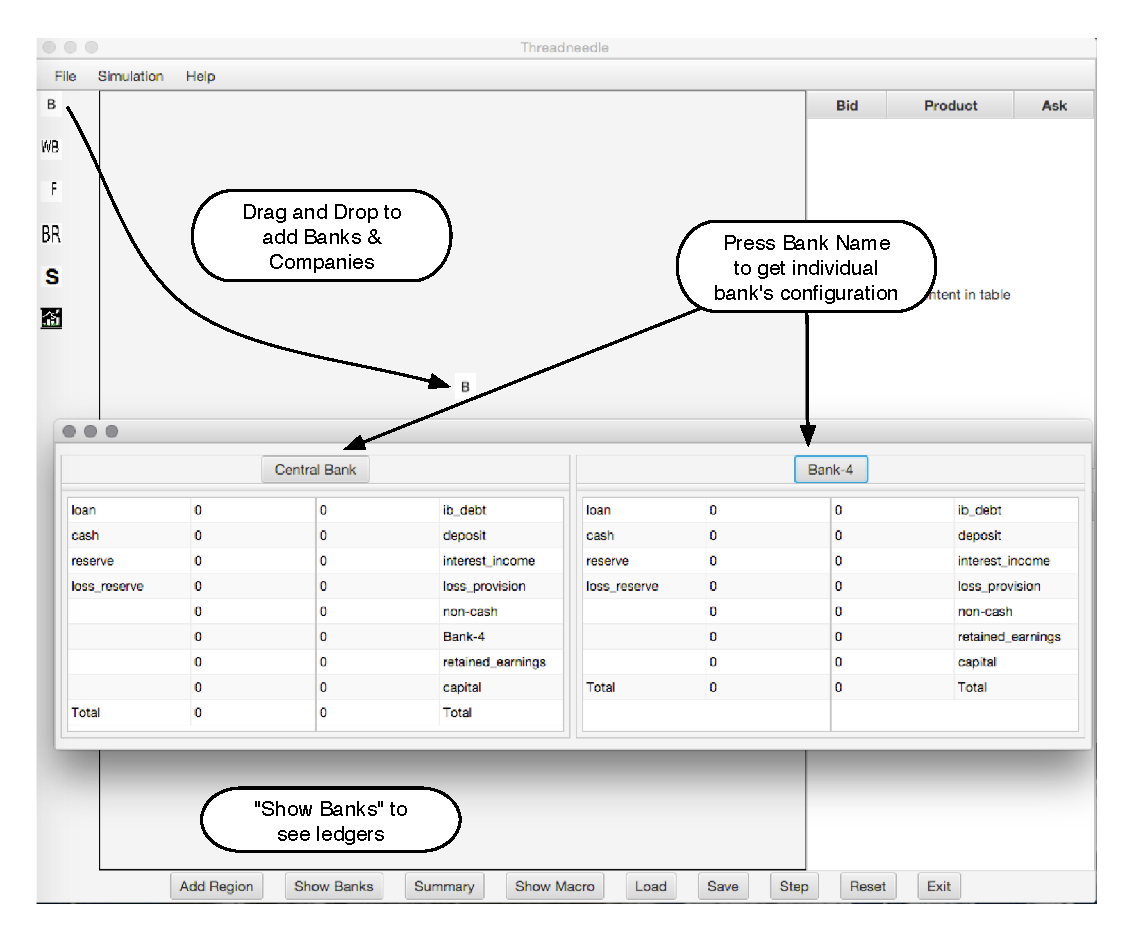
\includegraphics[width=12cm]{lab_fig_1.eps} 
\caption{Create Bank and Bring up Ledger}
\end{center}
\end{figure}

\begin{enumerate}
\item Add three banks to the Threadneedle simulation.
\item Use the "Show Banks" button to bring up the Bank balance display.
\item Using the guidelines below, configure the banks with identical
numbers of borrowers, capital, deposits, and reserves.
\begin{itemize}
\item The employer for each borrower should be the bank it has the deposit at.
\item Bank Capital should be added using the \emph{Investor} agent
\end{itemize}
\item \emph{Save the simulation.}
\item Run the simulation a few times to understand its behaviour.
\end{enumerate}

\subsection*{Bank setup}
For this simulation we will use the Borrower agent, which tries to take
out a loan, and if it suceeds repays the loan initially using loan funds,
and then a salary from the Bank. Borrowers effectively allow us
to isolate the banking system from its economy, and concentrate just
on banking mechanisms and lending flows.

However, the expansion from initial conditions does create some
challenges that require experimental design, otherwise we see
some rather strange effects. In particular, we
don't want all the loans to start at the same time, since this 
distorts the monetary behaviour of the system, and we need
to have adaquate cash and capital in the system to satisfy
regulatory requirements.

To even out lending over time, we can specify a Loan window.
The loan window setting controls when a borrower requests a loan.
So if we have a 12 period loan, and we set the loan window to 12,
the borrower will only request a loan every 12 steps. (The actual
step this occurs on is randomised.)

\subsection*{Guidelines}
\begin{itemize}
\setlength\itemsep{-0.5em}
\item[L =] Loan period in steps
\item[D =] Average loan amount
\item[R =] Central Bank Reserve requirement as a percentage.
\item[C =] Capital Reserve requirement as a percentage.
\end{itemize}

\begin{align*}
\text{Loan Window}  =& L \\[-0.5ex]
\text{No. of Borrowers} >=& 5*L \\[-0.5ex]
\text{Asset Cash} >=& L * D * R  \\[-0.5ex]
                  >=& Capital * C\\[-0.5ex]
\end{align*}

\begin{table}[h]
\centering
\begin{tabular}{lllll}
\multicolumn{5}{c}{Allocations} \\
\hline
Duration   & 12    & Asset Cash  & 12,000 &  \\
Reserve \% & .1    & Borrowers   &  60    &  \\
Window     & 12    & Deposit     &  100   &  \\
Loan       & 10000 & Investment  &  6000  &  \\
\end{tabular}
\end{table}
\section{Reserve vs Capital Regulation}
Reload the simulation defined above, and using the central bank 
configuration screen, enable capital controls. 

\begin{enumerate}
\item How does the system's behaviour change?
\item Increase the capital reserve requirement - what happens.
\item Turn on dividend payments on one of the banks - how does
its behaviour change with respect to the others?
\end{enumerate}

\section{Interbank Flows}
Reload the simulation defined above. Add a single additional
borrower to each bank, as follows: 

\begin{description}
\item[Bank 1] Add borrower with employer set to Bank 1 (control)
\item[Bank 2] Add borrower with employer set to Bank 2
\item[Bank 3] Add borrower with employer set to Bank 2
\end{description}

Run the simulation and observe what happens over time. Why?

\section{Financial Instruments}
Create a two bank system as above, with no interbank flows. 
Using the loan type, set
the borrowers of one bank to take out Compound interest rate
loans, and the other to take out Indexed Linked loans. 

How does the behaviour of the two banks differ?
\end{document}
